\section{evaluation}
\label{sec:evaluation}

In this section we introduce the evaluation result of our prototype implementation in Amazon EC2 public cloud.
The cloud environment is shown as Table.\ref{evaluation:amazon_environment}
\begin{table}[h]
\centering
\begin{tabular}{|c|c|}
Region				&		Tokyo		\\
Instance Type		&		m3.xlarge	\\
vCPUs				&		4			\\
ECUs				&		13			\\
Memory				&		15GiB		\\
Instance Storage	&		2*40GB(SSD)	\\
Network Performance	&		High		\\
\end{tabular}
\caption{evaluation environment}
\label{evaluation:amazon_environment}
\end{table}

\begin{table}[th]
\centering
\begin{tabular}{|c|p{150pt}|}
\hline
CPU					&		Intel\textregistered Core\texttrademark i7-3770K CPU @ 3.50GHz\\\hline
Memory				&		16GB\\\hline
Storage				&		Crucial m4 CT256M4SSD3 (256GB, mSATA)(Peak read: 500 MB/s, Peak write:260MB/s)*8\\\hline
RAID Card 			&		Adaptec ASR-7805Q Single\\\hline
RAID				&		Raid 0\\
\hline
\end{tabular}
\caption{stroage environment}
\label{evaluation:stroage_environment}
\end{table}

here vCPUs means the number of virtual CPU in instance, and one ECU provides the equivalent CPU capacity of a 1.0-1.2GHz 2007 Opteron or 2007 Xeon processor.

For the storage system, we used a machine inside our lab, the details is shows in
Table.~\ref{evaluation:stroage_environment}.

All the compute nodes, I/O nodes and master node connect with interconnection network inside Amazon
EC2, and mount storage system by sshfs\cite{sshfs} via Internet.

\subsection{One User Performance}

\begin{figure}
\centering
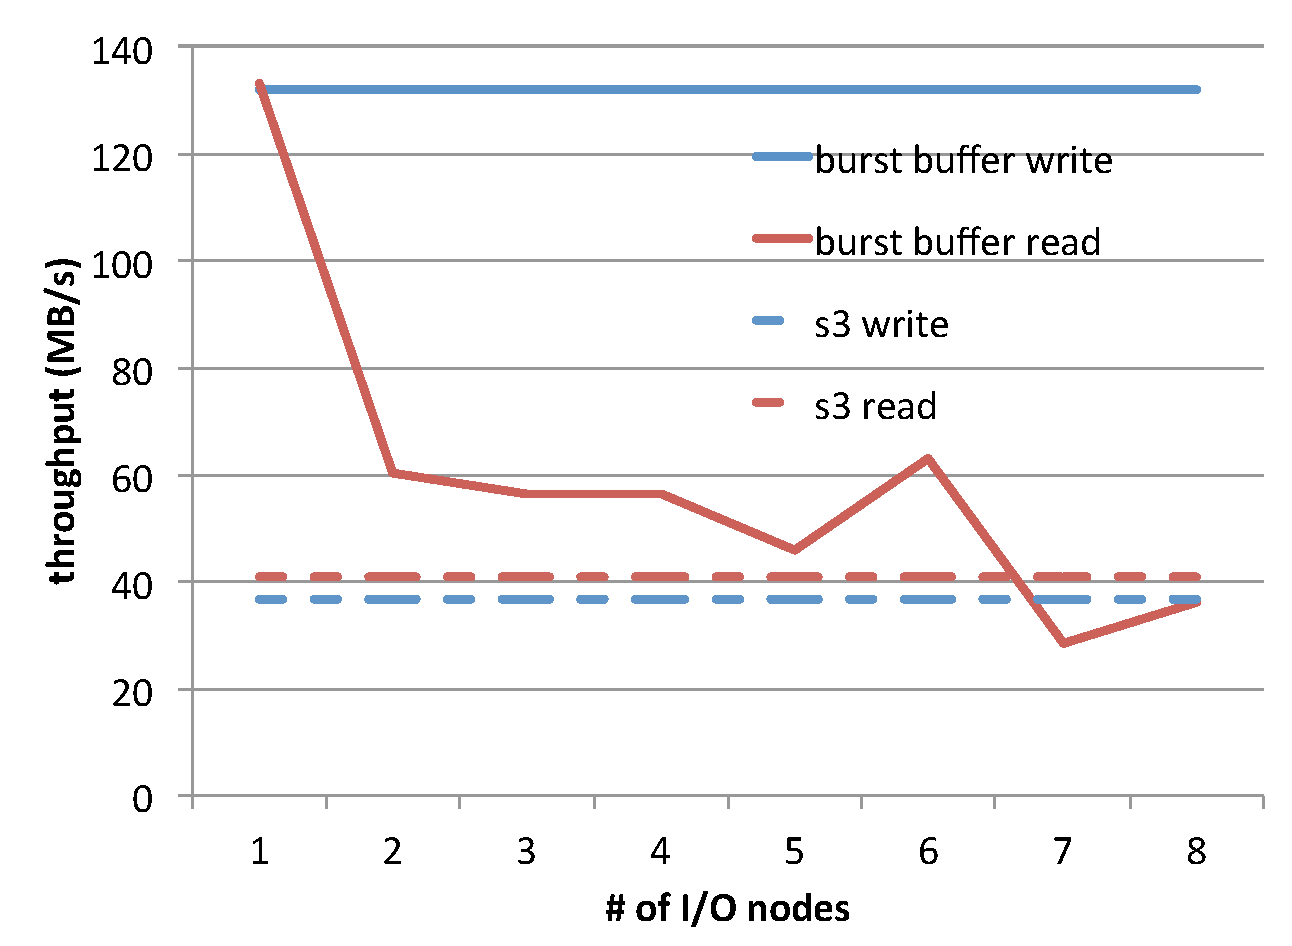
\includegraphics[width=8.5cm]{img/one_client.pdf}
\caption{One User Performance}
\label{evaluation:one user performance}
\end{figure}

First we measure the performance of our prototype for only one user, and shows how our system
will affect one user performance.
In this experiment, the number of client is fixed to one, and measure
the sequential read and write performance for different number of I/O nodes.
All I/O data are distributed among all I/O nodes.
Figure~.\ref{evaluation:one user performance} shows one user performance.
As we know, one thread I/O is difficult to achieve the full throughput on Internet, we can see from
Figure.~\ref{evaluation:one user performance} that without I/O node, applications can only achieve a
throughput under 20MB/s in reading and under 80MB/s in writing.

However by using our system the read throughput increasing as the number of I/O nodes, and can
achieve about 8 times faster than the throughput without I/O nodes.
For writing throughput, the interconnection throughput is different from Internet throughput, it can
achieve full throughput even with one thread, but the throughput is limited by the client node
throughput which is also 1Gbps(135MB/s).

\subsection{Multiple Users Performance}

\begin{figure}
\centering
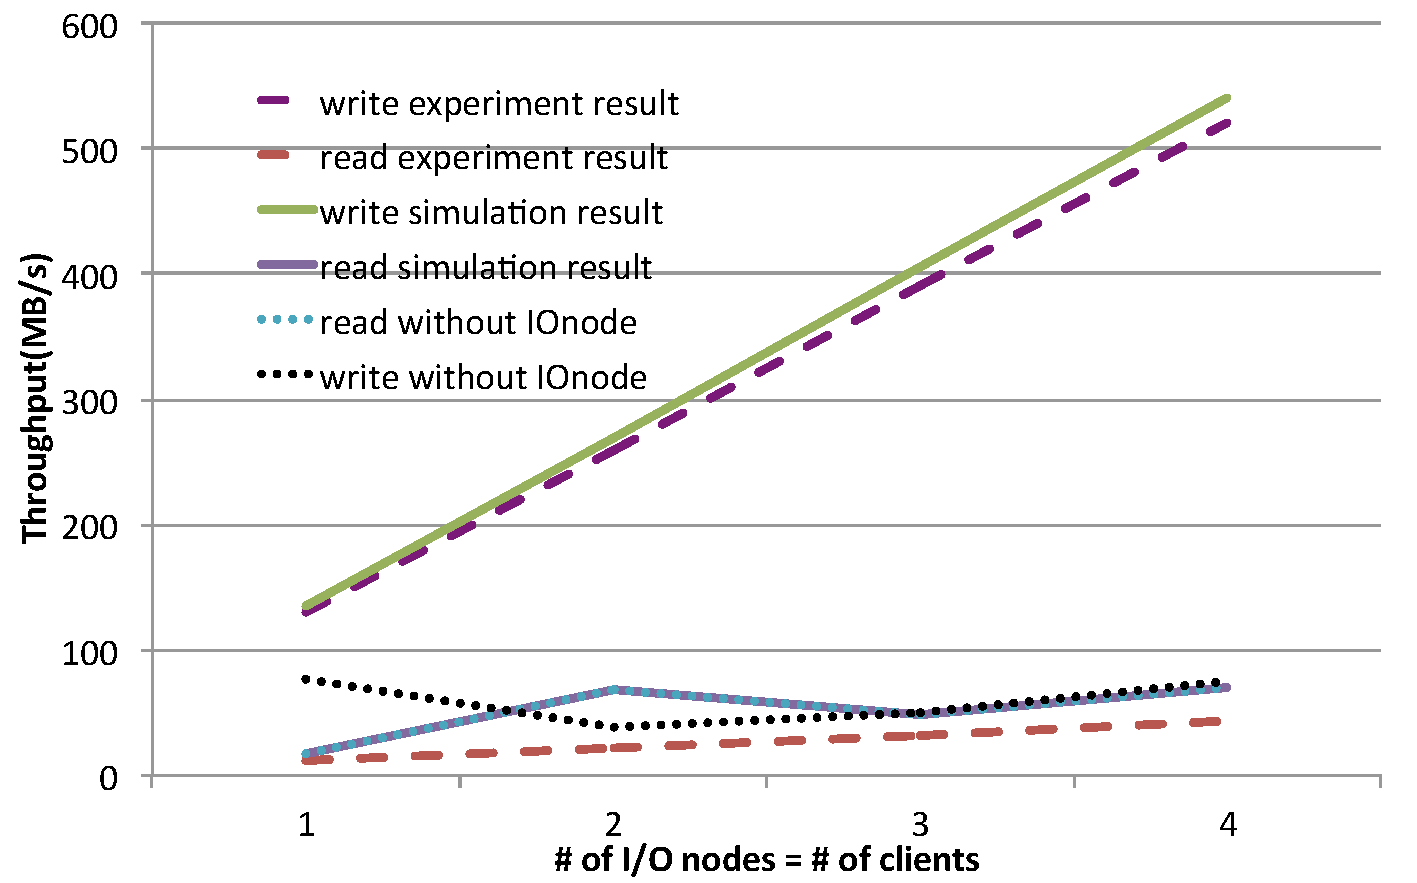
\includegraphics[width=8cm]{img/multiple_client.pdf}
\caption{Multiple User Performance}
\label{evaluation:multiple user performance}
\end{figure}

In the second experiment, we measured the throughput of multiple clients.
To simplified the experiment, we assume that one client connect to only one I/O nodes, and one I/O
nodes buffer all the I/O data for a client.
Figure.~\ref{evaluation:multiple user performance} shows the overall throughput of the whole system.
Since all the data are stored on the shared storage, and need to be transferred via Internet, the
read throughput doesn't change by using I/O nodes.
However when we look at the write throughput, it shows a strong scalability, and achieved 7 times
improvement with only 4 I/O nodes.

\subsection{Simulation for Applications}
Show our architecture can burst I/O performance for applications
x